\chapter{Anhang}
\label{appedixa}
\begin{figure}[h]
	\centering
		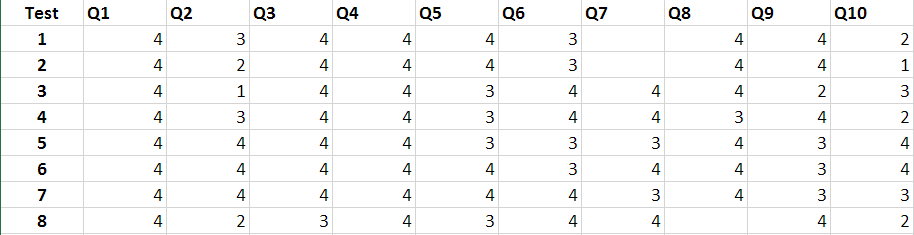
\includegraphics[width=1.00\textwidth]{media/tableData.png}
	\caption{Datenreihe von Fragebogen A}
	\label{fig:tableData}
\end{figure}

\clearpage

%*********************************************************************%
% Dokumente                                                           %
%*********************************************************************%
\refstepcounter{section}
\addcontentsline{toc}{section}{\protect\numberline{\thesection} Fragebogen A}
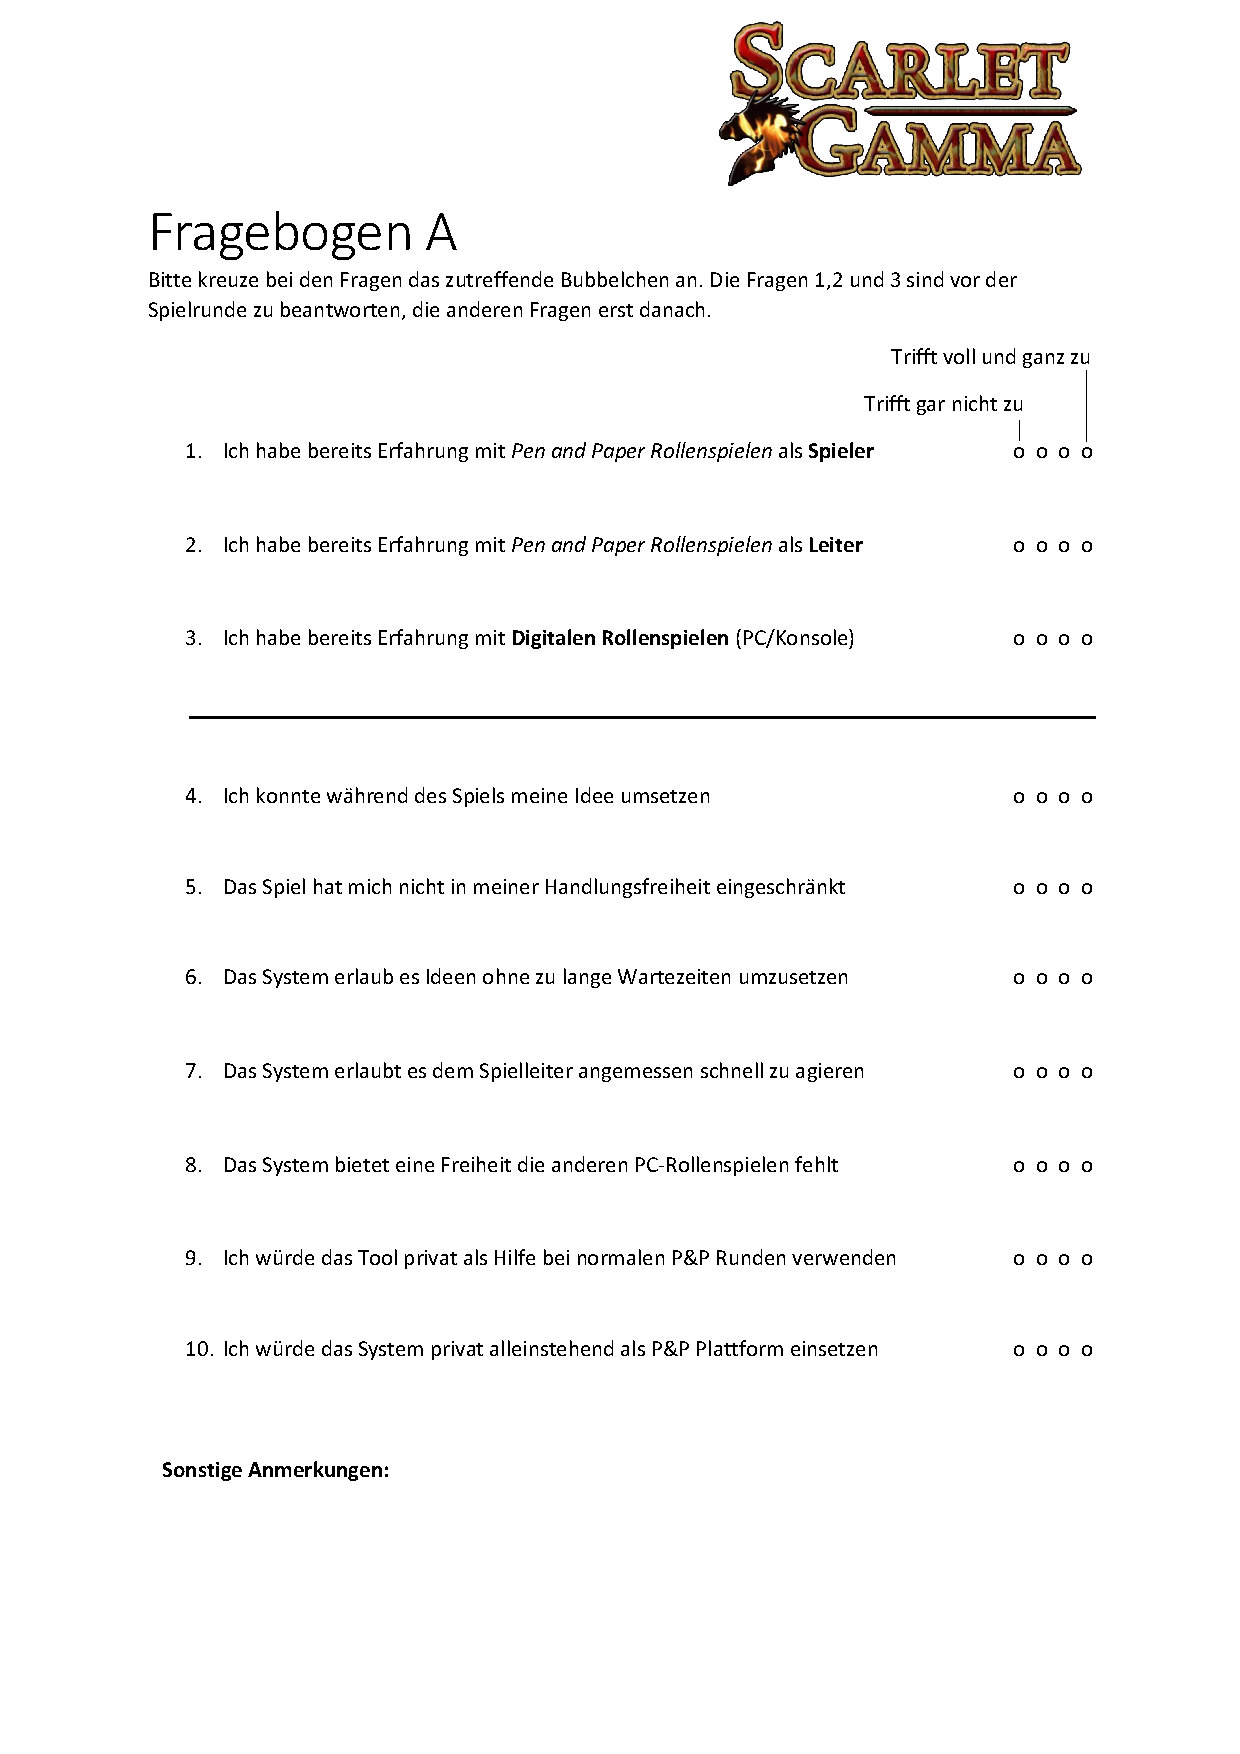
\includepdf[pages=-,link,linkname=AppendixFragebogenA]{../Fragebogen_A.pdf}
\refstepcounter{section}
\addcontentsline{toc}{section}{\protect\numberline{\thesection} Testszenario Spielleiter}
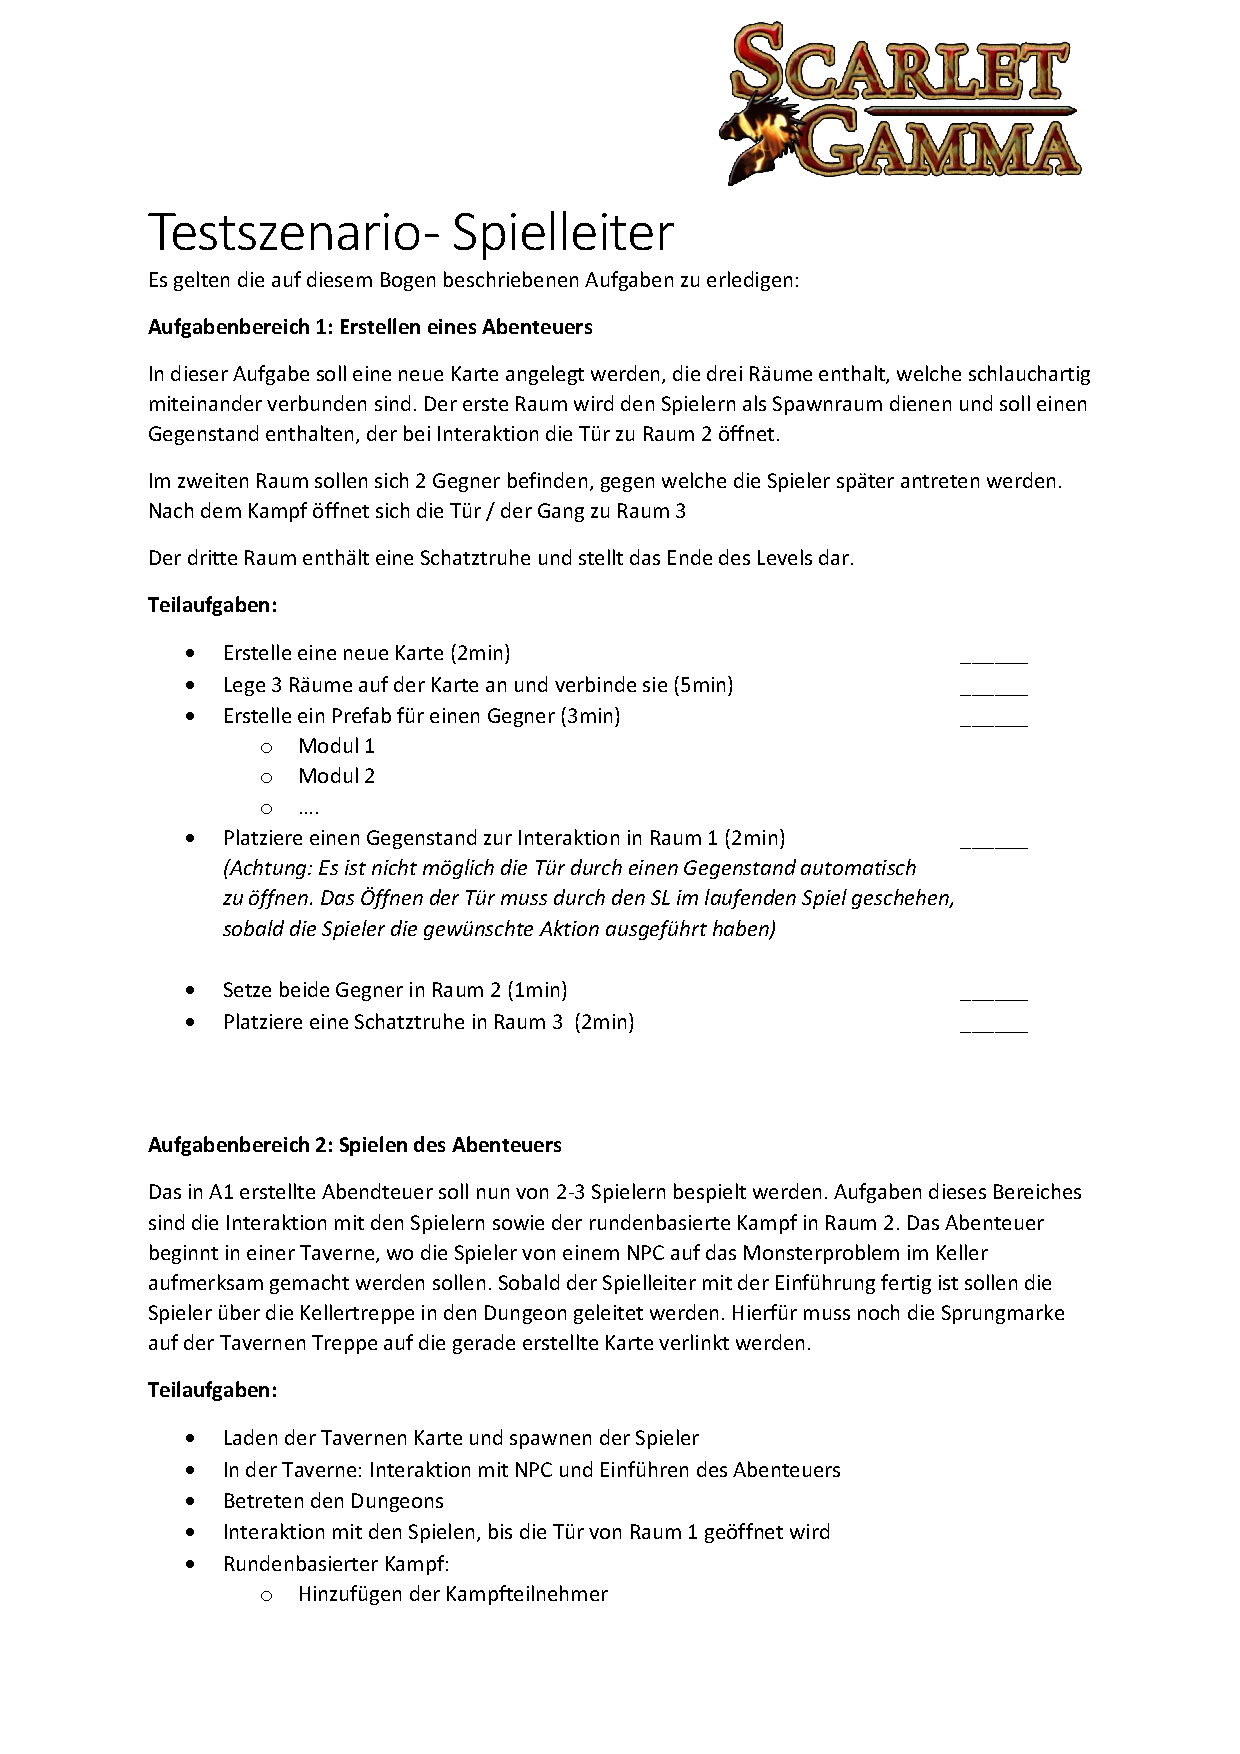
\includepdf[pages=-,link,linkname=AppendixSpielleiter]{../Testszenario_Spielleiter.pdf}
\refstepcounter{section}
\addcontentsline{toc}{section}{\protect\numberline{\thesection} Handbuch}
\includepdf[pages=-,link,linkname=AppendixManual]{../QuickManual/manual.pdf}
